\section{Description of Tool}
\label{sec:tool}

\begin{figure}[ht]
  \centering
  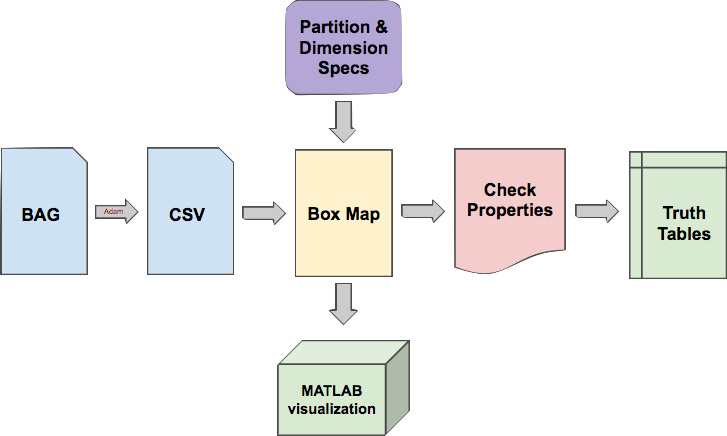
\includegraphics[width=0.95\textwidth]{./figures/workflow}
  \caption{Overview of tool workflow.}
  \label{fig:workflow}
\end{figure}

% since we're considering cubes we only need a desired cube size, no need for partitions
Our tool will take trace files, a cube size, and bounding dimensions as input, and will return a set of spatial-temporal properties inferred from the traces.  

 This description elaborates on the high-level workflow diagram.
The trace files will be one or more .bag files.  
A bag is the file format used by the Robot Operating System (ROS) for storing ROS message data.  
Via messages, various sensors can write their values to these bags during an execution. 
These values may be examined after any run.
In our current implementation, we are only considering the values of time stamps and x, y, and z positions.

We first convert the .bag files to .csv files with four columns which contain a timestamp and the associated x, y, and z position values (in meters).  
 Our tool currently makes the assumption that we receive one \emph{complete} trace of some run, so we are not stitching together partitions of lengthy runs; this may need to be done in the future.
 Each time frame is mapped to some box, so to temporally sync the runs, we are considering the start of the run to be the global time frame of the greatest initial time frame of all given traces.

The cube size is given as a single positive floating-point integer, representing the desired length of the cube edge in meters.
The bounding dimensions are given as a 3-tuple of positive floating-point integers, representing the bounds of the space in which the actors move.
Given the cube size, we map the position of each time frame of a single trace to the box corresponding to its position in $R^3$.
 This produces a total ordering of abstracted trace positions given as a succession of boxes, which we will call a box-trace.
 
 Additionally, you need to set a flag to indicate if the input deals with a single actor or multiple actors.
 
 Based on a set of box-traces, we will check if certain properties hold.
 For example, if a trace starts out in "box 3," moves to other boxes, and occupies "box 3" at a later time, then the return home property would be set to true.
 
 The output will be a set of one or more truth tables corresponding to a subset of the properties discussed in methods.
 The format of these truth tables is also discussed in methods.
 You may optionally output a 3D visualization of the box-trace, displayed in MATLAB.
 
 For many of the above properties, it will be important to know specific details of violated properties (which box, which time frame, etc.); these details are being stored but we are currently only outputting binary truth values. 
 
 % to go in methods section?
 Let there be $m$ properties.
 If we are considering a single actor, the truth table will just be one row with $m$ columns containing the truth value of the corresponding property.
 If we are considering $n$ multiple actors, the output will be $m$ truth tables which are either $1 \times n$ or $n \times n$ matrices, depending on the property considered.
 For example, the returns home property only depends on a single actor, not their interactions, so the table will be a $1 \times n$ matrix with the truth value of each actor.
 But a property like box-independence considers interactions between all the actors, and so its truth table will be a $n \times n$ matrix with the truth value for box-independence between $(box_i,box_j)$ for all $1 \leq i,j \leq n$.

% \begin{itemize}
% \item \emph{Input}: 
%   \begin{itemize}
%    \item One or more .bag files of ROS message data containing positional data and time stamps
%    \item A flag to indicate a single actor or multiple actors
%    \item Partition specifications given as a 3-tuple of positive integer values
%    \item Dimension specifications (in meters) given as a 3-tuple of positive floating-point values
%   \end{itemize}

%  \item \emph{Output}:
%   \begin{itemize}
%    \item Visualization in MATLAB of actor's/actors' movement through space
%    \item Truth table(s) with the following properties:
%      \begin{itemize}
%       \item moves? : occupies more than one box
%       \item returns home? : occupies the initial box in separate time intervals
%       \item box independence? : multiple actors (traces, given a single actor) never occupy the same box simultaneously
%       \item crumb independence? : multiple actors (traces, given a single actor) never cross each other's box-path
%       \item fuzzy box independence? : multiple actors (traces, given a single actor) never occupy the same "fuzzy" box simultaneously
%       \item fuzzy crumb independence? : multiple actors (traces, given a single actor) never cross each other's "fuzzy" box-path
%       \item returns to some box? : occupies the same box in separate time intervals
%       \item loiters? : remains in the same box for more than 30 seconds
%      \end{itemize}

%   \end{itemize} 
% \end{itemize}
